\documentclass[sigconf,nonacm]{acmart}
% Standalone build. Venue/format not yet chosen; nonacm removes ACM
% rights/venue metadata. Retarget by swapping the documentclass options.
\usepackage{booktabs}
\usepackage{graphicx}

\settopmatter{printacmref=false}
\setcopyright{none}
\acmDOI{}
\acmISBN{}

\newcommand{\ctx}{\texttt{context.md}}
\newcommand{\artifact}{\url{https://github.com/kerbelp/context-md}}

\begin{document}

\title{Context Inheritance: Capability-Dependent Benefits of Repository
Context for AI Coding Agents}

\author{Pavel Kerbel}
\authornote{Corresponding author. All authors are affiliated with Metatron Research (\url{https://getmetatron.com}); ORCIDs identify each author.}
\orcid{0009-0004-4679-1036}
\email{pavel@getmetatron.com}
\affiliation{\institution{Metatron Research}\country{}}
\author{Milana Kerbel}
\orcid{0009-0004-7893-9824}
\email{milana@getmetatron.com}
\affiliation{\institution{Metatron Research}\country{}}
\author{Vitali Abramov}
\orcid{0009-0007-0814-3822}
\email{vitali@getmetatron.com}
\affiliation{\institution{Metatron Research}\country{}}
\author{Liat Abramov}
\orcid{0009-0006-1601-146X}
\email{liat@getmetatron.com}
\affiliation{\institution{Metatron Research}\country{}}

\begin{abstract}
Giving an AI coding agent a repository's operating context---its decisions,
constraints, and conventions---sometimes helps a great deal and sometimes not
at all. We show the difference is governed by a single variable: the capability
of whoever \emph{wrote} the context relative to the agent that \emph{reads} it.
Across pre-registered experiments on SWE-bench Verified spanning a small local
executor (Gemma~3, 8B) and a frontier executor (Claude Opus 4.8), a repository
context layer raises a weak reader's gold-file localization by 26 percentage
points ($p<0.0001$) when the context was authored by a more capable model, and
by exactly nothing ($+0.0$~pp, $p=1.0$) when the reader authored it itself. The
benefit is a capability \emph{threshold}, not a dose curve: any author above the
reader roughly doubles the reader's localization; a self-taught weak model
equals no context. At the top of the range the picture inverts along a second
axis---\emph{what} transfers. A frontier agent gains from its own
failure-derived lessons (+14.6~pp resolve on constraint-sharing tasks,
$p=0.041$; $-32\%$ tokens per resolved task) but nothing from answer-derived
summaries, while a weak model benefits most from exactly those summaries. On a
broad random sample the frontier agent sits at a resolve ceiling (91\% with no
context) that no delivery mechanism improves, and where reading a context store
only adds token cost. We call the organizing principle \emph{context
inheritance}: repository context is senior knowledge that propagates
\emph{down} a capability gradient. The practical rule follows directly---seed and
maintain context layers with the most capable available author, and expect the
benefit to accrue to the cheaper agents that read them.
\end{abstract}

\keywords{AI coding agents, repository context, capability gradient, knowledge
transfer, SWE-bench, pre-registered study}

\maketitle

\section{Introduction}
A modern coding agent, handed a bug, can plan, edit, run tests, and iterate for
hours. What it cannot do is know the things a repository never wrote down: which
library the team removed and why, which layering rule is unwritten, which
approach looks reasonable but was tried and rejected. A \emph{repository context
layer}~\cite{manifesto,rcl}---a small, version-controlled, human-readable store
of a project's operating context, consulted by the agent before it acts---is one
answer to this gap. But a practitioner who adopts one quickly meets a confusing
fact: sometimes it transforms the agent's behavior, and sometimes it does
nothing at all.

This paper explains the variance. We find that the benefit an agent draws from
repository context is \emph{capability-dependent}: it is a function of how
capable the context's author was relative to the agent reading it. When a
stronger author writes for a weaker reader, the reader inherits a large,
statistically decisive navigational benefit. When author and reader are the same
weak model, the benefit is exactly zero. And when the reader is already a
frontier model operating near its ceiling, generic context adds no resolution
and only spends tokens.

We establish this across a family of pre-registered experiments on SWE-bench
Verified~\cite{swebench}, varying three factors independently: the \emph{executor}
(a small local model, Gemma~3~8B, and a frontier model, Claude Opus 4.8); the
\emph{author} of the context (none; the executor itself; a more capable model
writing blind; and a labeled oracle bound); and the \emph{delivery} mechanism
(injected into the prompt, a monolithic file, or a sharded store the agent reads
selectively). Our contributions are:

\begin{enumerate}
\item \textbf{A capability gradient in context benefit.} With the executor held
fixed at 8B, a blind frontier-authored seed raises gold-file localization from
21.1\% to 47.2\% ($+26.1$~pp, $p<0.0001$), while the executor's own promoted
lessons move it not at all ($+0.0$~pp, $p=1.0$). The effect is a threshold:
context helps iff its author outranks its reader (Section~\ref{sec:gradient}).
\item \textbf{An inversion in what transfers, by reader capability.} A weak
reader benefits most from answer-derived summaries (where things are); a frontier
reader benefits only from its own failure-derived lessons (where it will go
wrong), gaining $+14.6$~pp resolve on constraint-sharing tasks ($p=0.041$)
(Section~\ref{sec:whattransfers}).
\item \textbf{A frontier ceiling, and the cost of context there.} On a broad
random sample the frontier executor resolves 91\% of well-specified bugs with no
context; no delivery mechanism improves this, and the selective store costs more
tokens, not fewer, at high capability (Section~\ref{sec:ceiling}).
\item \textbf{Token economics of inheritance.} Where context does help a capable
reader, it pays for itself: $-32\%$ tokens per resolved task
(Section~\ref{sec:tokens}).
\end{enumerate}

The synthesis is a design principle we call \emph{context inheritance}:
repository context behaves like senior engineering knowledge, and its value
propagates \emph{down} a capability gradient---from a strong author, once, to
every cheaper agent that later reads the repository.

\section{Background}
Teams already convey project knowledge to agents through instruction files
(\texttt{CLAUDE.md}, \texttt{AGENTS.md}), IDE memories, and
retrieval-augmented generation. A repository context layer differs in being
co-versioned with the code, human-reviewed, and consulted by contract rather
than by retrieval similarity; the architecture and its properties are specified
elsewhere~\cite{manifesto,rcl} and are not the subject of this paper. Our
question is narrower and empirical: \emph{given} such a layer, what determines
whether an agent benefits from it? Prior agent-memory work (Reflexion,
Voyager, MemGPT, Generative Agents~\cite{reflexion,voyager,memgpt,genagents})
studies a single agent accumulating its own experience. The phenomenon we isolate
is cross-capability: knowledge written by one model and read by another, of
different strength.

\section{Method}
The protocol (hypotheses, conditions, metrics, analysis plan, power simulation)
was pre-registered and externally timestamped at a git tag before any
confirmatory run; pilot runs are excluded from confirmatory analysis. All
materials---the frozen protocol, the blind-authoring audit, episode transcripts,
promotion logs, and containerized evaluation verdicts---are released for
replication~\cite{artifact}.

\emph{Executors.} A small local model (Gemma~3, 8B, quantized) and a frontier
model (Claude Opus 4.8), each run in an identical minimal agent scaffold: read
files, edit code, run individual tests, up to a fixed turn budget, leaving an
uncommitted working-tree patch. Every episode is a fresh model session in a
freshly cloned checkout; no state carries between episodes.

\emph{Context authors.} Context is \emph{none}; authored by the executor itself
through a consult--execute--learn--promote lifecycle (self-authored); authored
by a more capable model given only a years-old, history-stripped checkout and
constraint-group names, never a problem statement, patch, or test (a blind seed);
or authored with sight of the maintainers' gold patch (a labeled oracle bound,
never pooled with confirmatory arms). Crucially, \textbf{no context was produced
by an automatic extraction pipeline}: all authored context is blind or
lifecycle-derived by design, so that the study isolates the capability-of-author
effect and cannot leak held-out solutions. Automatic extraction is deferred to
future work (Section~\ref{sec:threats}).

\emph{Delivery.} Where context is present it is delivered as an injected prompt
block, a single monolithic \ctx{} the agent is instructed to read, or a
\emph{sharded} store (an index plus one file per decision) the agent reads
selectively under a consultation contract.

\emph{Instances and metrics.} Two instance regimes are used and never conflated:
ordered \emph{transfer pairs} $(A,B)$ within a repository whose fixes depend on
the same constraint (the regime the layer is designed for, about 8\% of
Verified), and a broad stratified random sample. Metrics: \emph{consultation}
(did the agent read the context, from transcripts), \emph{gold-file localization}
(did it edit a file the maintainers' fix touched), \emph{resolve} (did its patch
pass the hidden test suite, via the official SWE-bench containers), and
\emph{tokens} per episode and per resolved task. Paired comparisons use sign-flip
permutation tests (10k draws, fixed seed); families are Holm-corrected.

\section{The capability gradient}\label{sec:gradient}
Holding the executor fixed at 8B (36 transfer pairs $\times$ 5 repetitions =
180 held-out episodes per arm), the held-out outcome varies only with who
authored the context (Figure~\ref{fig:gradient}).

\begin{table}[t]
\caption{Weak executor (8B), held-out localization by context author. 180
episodes/arm.}
\label{tab:gradient}
\begin{tabular}{lccc}
\toprule
context author & non-empty & gold-hit & resolve \\
\midrule
none & 68.3\% & 21.1\% & 5.6\% \\
self-authored (8B) & --- & 21.1\% & --- \\
blind frontier seed & 81.1\% & \textbf{47.2\%} & 6.1\% \\
gold-distilled (oracle bound) & 79.4\% & \textbf{42.8\%} & 7.8\% \\
\bottomrule
\end{tabular}
\end{table}

\begin{figure}[t]
\centering
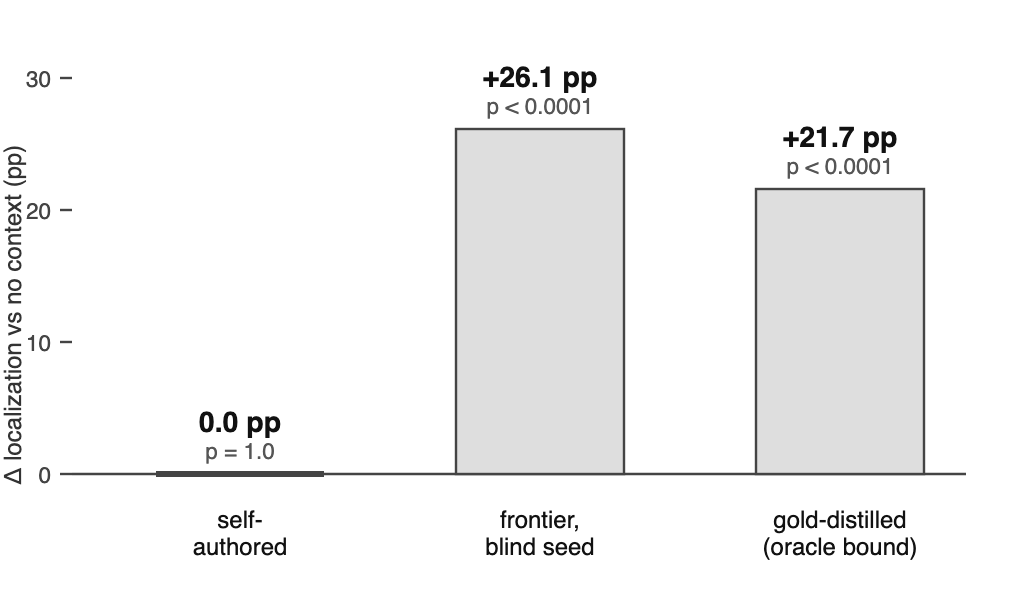
\includegraphics[width=\columnwidth]{figures/fig1-gradient.png}
\caption{Paired improvement in the 8B executor's gold-file localization over its
no-context control, by context author (36 pairs $\times$ 5 repetitions).
Self-authored context moves nothing; any author more capable than the reader
roughly doubles localization. Resolve-rate deltas are not significant at this
tier.}
\label{fig:gradient}
\end{figure}

A blind frontier-authored seed raises gold-file localization from 21.1\% to
47.2\%---$+26.1$~pp, paired $p<0.0001$, far beyond the pre-registered minimum
detectable effect. Gold-distilled context, an upper bound, raises it to 42.8\%
($+21.7$~pp, $p<0.0001$); the two capable-author tiers are statistically
indistinguishable. The executor's \emph{own} promoted lessons---162 of them
across 60 pair-repetitions---move localization by $+0.0$~pp ($p=1.0$): exactly
the no-context control.

Two readings are ruled out. This is not a dose curve in which more capable
authorship yields proportionally more benefit; blind-seed and oracle are a tie,
so the shape is a \emph{threshold}---context helps if and only if its author
outranks its reader. And it is not that the 8B model cannot use context: it uses
frontier-written context decisively; it simply cannot \emph{write} context worth
reading. Inspection of the self-authored store shows why: the weak model records
tooling tactics (``run pytest with \texttt{-x}''), not repository constraints,
whereas the frontier author, under the identical learning prompt, records the
constraint-and-localization facts the transfer clusters center on.

At this tier the movement is in localization and episode completion, not resolve:
all arms sit at 5--8\% resolve, and no resolve claim is supported (the pooled
oracle delta is $+2.2$~pp, $p=0.22$). Localization is a proxy for working in the
right place, not for correctness; we report it as such.

\section{What transfers depends on the reader}\label{sec:whattransfers}
The gradient says a capable author helps a weak reader. At the top of the range,
a second axis appears: \emph{what kind} of knowledge transfers depends on the
reader's capability.

Running the full consult--execute--learn--promote lifecycle with the frontier
executor on 16 constraint-sharing pairs ($\times$ 3 repetitions, 48 held-out
episodes/arm), the agent's own failure-derived lessons---extracted from working
task $A$, never seeing a gold patch or hidden test---raise held-out resolve on
task $B$ from 58.3\% to 72.9\%: $+14.6$~pp, paired $p=0.041$, the frontier-tier
pre-registered primary. Yet lessons distilled from the \emph{gold patch} of task
$A$ transfer nothing at this tier (60.4\% resolve, indistinguishable from no
context).

This is the exact inverse of the weak tier, where gold-distilled context was the
\emph{strongest} author. The interpretation is sharp: answer-derived lessons
encode solutions; failure-derived lessons encode traps and process. A weak model
needs to be told where things are; a strong model already localizes and instead
needs to be told where it will go wrong. For context-layer design this means the
transferable payload changes with the reader---solution summaries for weak
readers, process and failure knowledge for strong ones.

\section{The frontier ceiling}\label{sec:ceiling}
Both results above use constraint-sharing pairs, the regime a context layer is
built for. What happens when a frontier agent meets a \emph{broad} random sample
with generic repository context? We ran all four delivery conditions---no context
(B), injected (E), monolithic file (FILE), and sharded store (SHARD)---with the
frontier executor on an 88-instance stratified subset of Verified, one repetition
(Table~\ref{tab:ceiling}).

\begin{table}[t]
\caption{Frontier executor (Opus 4.8), broad 88-instance sample. Consultation is
the fraction of episodes that read the context; cost is notional, at list prices,
excluding prompt caching.}
\label{tab:ceiling}
\begin{tabular}{lcccc}
\toprule
delivery & resolve & consult & prompt-tok & \$/resolved \\
\midrule
none (B) & \textbf{90.9\%} & 0\% & 25.8K & 0.153 \\
injected (E) & 81.8\% & 0\% & 23.5K & 0.157 \\
file (FILE) & 85.2\% & 100\% & 24.0K & 0.154 \\
sharded (SHARD) & 88.6\% & 100\% & 38.4K & 0.230 \\
\bottomrule
\end{tabular}
\end{table}

Two facts stand out. First, the no-context baseline already resolves 90.9\% of
these well-specified, isolated bugs: the frontier model does not need repository
context to fix bugs it can already localize, and there is no headroom for context
to add resolution. No delivery mechanism beats the baseline; the small
differences among B/E/FILE ($\pm$ a few instances on $n=88$) are within noise.
Second, the consultation contract binds perfectly---FILE and SHARD read the
context in 100\% of episodes---so the null is not a failure to read; it is that
reading generic context on a random bug has nothing to contribute.

The ordering among the context arms is nonetheless consistent with the weak-tier
finding that \emph{selection beats volume}: injecting the whole payload (E,
81.8\%) hurts most, selective reading (SHARD, 88.6\%) hurts least, monolithic
reading (FILE, 85.2\%) sits between. But at frontier capability the selective
store's cost \emph{inverts}: a capable model turns ``read only what you need''
into thorough exploration, so SHARD spends 38.4K prompt tokens against FILE's
24.0K and costs $\sim$50\% more per resolved task. At the weak tier the same
sharded store was the \emph{cheapest} arm, paying roughly three times fewer
context tokens than the monolith. Selection is economical for readers that read
sparingly; a strong reader reads thoroughly.

Together with the gradient, this completes the capability story: context benefit
requires an author above the reader \emph{and} a reader below its ceiling. A
frontier model on a broad, well-specified bug set violates the second condition,
and generic context becomes a cost rather than a benefit.

\section{Token economics}\label{sec:tokens}
Where context does help a capable reader---the constraint-sharing regime of
Section~\ref{sec:whattransfers}---it is self-financing (Figure~\ref{fig:tokens}).
The self-taught frontier lifecycle spends 55.7K tokens per resolved task against
81.8K with no context: $-32\%$. The decomposition is instructive: episodes that
end in a fix cost about the same in both arms ($\sim$33.6K); the savings come
entirely from fewer doomed explorations. Context of any kind shortens wandering
(the oracle arm saves tokens identically), but only failure-derived context also
converts the saved effort into additional resolves. For a strong reader in the
right regime, context is paid back in tokens; for a weak reader it is a paid
navigational upgrade (the injected block costs $+20\%$ tokens per episode even as
it shortens episodes).

\begin{figure}[t]
\centering
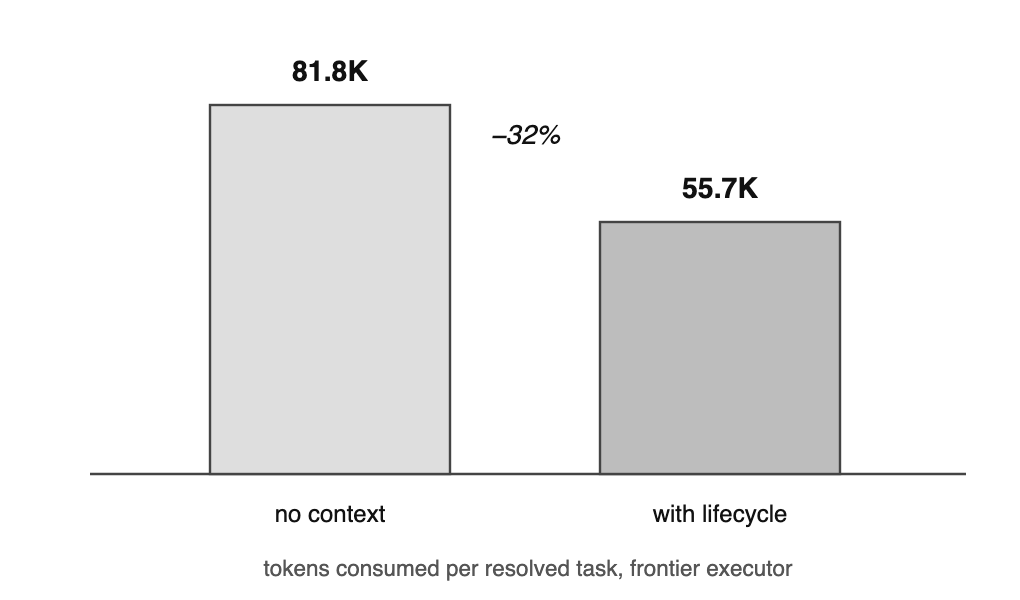
\includegraphics[width=\columnwidth]{figures/fig2-tokens.png}
\caption{Frontier executor, constraint-sharing regime: tokens consumed per
resolved task, no context vs.\ the self-taught lifecycle. The saving is from
fewer failed explorations, not cheaper fixes.}
\label{fig:tokens}
\end{figure}

\section{Discussion: context inheritance}
The four results resolve into one principle. Repository context is not a uniform
good that any agent draws on equally; it is \emph{senior knowledge}, and its
value flows down a capability gradient. A reader inherits benefit in proportion
to how far its context's author outranks it, and only while the reader has
headroom to improve. This reframes several practical questions:

\emph{Who should write the context?} The most capable author available---a
human expert, a frontier model, or distillation from authoritative fixes. A
project should not rely on its cheap working agents to author their own context;
a weak self-taught loop equals no context exactly.

\emph{Who benefits?} The cheaper agents. One frontier authoring pass, paid once,
propagates senior-level navigational knowledge to every local agent that later
reads the repository at zero marginal inference cost. This is the economic case
for the pattern: expensive knowledge, written once, read cheaply forever.

\emph{When is it worth it?} When the reader is below its ceiling on the task
distribution---weaker models broadly, and strong models on tasks that are
ambiguous, convention-laden, or re-hit a known constraint. On well-specified
bugs a frontier model already resolves, generic context is not worth its token
cost.

\section{Threats to validity}\label{sec:threats}
\emph{Benchmark scope.} SWE-bench Verified supplies well-specified, isolated bug
fixes graded by hidden tests. It cannot measure a context layer's central
real-world value---adherence to conventions and avoidance of rejected
approaches, where ``correct'' is not ``tests pass.'' The frontier ceiling of
Section~\ref{sec:ceiling} is therefore a statement about this task type, not
about repository context in general; a benchmark that scores
convention-adherence is needed to probe the value the frontier ceiling hides,
and is the natural next instrument.

\emph{Extraction untested.} All authored context here is blind- or
lifecycle-derived, deliberately, to isolate the author-capability effect and
guarantee no leakage of held-out solutions. Whether an automatic extraction
pipeline can \emph{produce} context of comparable value is a separate question
this design brackets; it is the clearest follow-up---vary the context's
\emph{author} (blind-frontier vs.\ machine-extracted vs.\ human-curated) with
delivery and executor fixed.

\emph{Statistical scope.} The frontier resolve effect ($n=16$ pairs $\times$ 3)
and the broad-sample matrix ($n=88$, one repetition) have wide intervals; the
gradient and its threshold shape, pooled to 180 episodes/arm, are the robust
core. Contamination affects both arms of every within-model comparison
symmetrically, compressing deltas toward zero. Transfer pairs target
constraint-shaped bugs by construction---construct validity, since recurring
constraints are the only setting in which shared context can pay off.

\section{Conclusion}
Whether a repository context layer helps an AI coding agent is not a property of
the layer alone; it is a relation between the capability of the context's author
and the capability of its reader. A stronger author lifts a weaker reader
decisively---doubling its localization---while a self-taught weak model gains
nothing and a ceilinged frontier model gains nothing generic delivery can add.
Context flows down the capability gradient. The design consequence is concrete:
author repository context with the strongest writer you have, and reap the
benefit in every cheaper agent that reads it.

\section*{Conflicts of Interest}
All authors are affiliated with Metatron Research, whose open-source
implementation of the repository-context pattern (Metatron) motivates this study.
The experiment mitigates this competing interest by pre-registration before data
collection, a scaffold-uniform minimal harness rather than the product itself,
context that is blind- or lifecycle-authored rather than produced by that
implementation, and fully public data and analysis code.

\section*{AI-Assisted Preparation Statement}
Consistent with COPE guidance, the authors disclose that large language models
(Anthropic Claude) were used to assist with manuscript drafting, analysis
scripting, and experiment orchestration, under continuous author direction and
review. The authors take full responsibility for the final text and all reported
results.

\section*{Data Availability}
The frozen pre-registration, blind-authoring audit, episode transcripts,
promotion logs, containerized evaluation verdicts, and analysis scripts are
released for replication~\cite{artifact}.

\begin{thebibliography}{9}
\bibitem{manifesto} P.~Kerbel. ``The Repository Context Layer: The Missing Layer
of Agentic Software Development,'' manifesto and specification, 2026.
\url{https://github.com/kerbelp/repository-context-layer}.
\bibitem{rcl} P.~Kerbel, M.~Kerbel, V.~Abramov, and L.~Abramov. ``The Repository
Context Layer: A Git-Native Architecture for AI Coding Agents,'' 2026.
\bibitem{swebench} Carlos E. Jimenez, John Yang, Alexander Wettig, Shunyu Yao,
Kexin Pei, Ofir Press, and Karthik Narasimhan. 2024. SWE-bench: Can Language
Models Resolve Real-World GitHub Issues? In \emph{ICLR 2024}.
\bibitem{reflexion} Noah Shinn, Federico Cassano, Ashwin Gopinath, Karthik
Narasimhan, and Shunyu Yao. 2023. Reflexion: Language Agents with Verbal
Reinforcement Learning. In \emph{NeurIPS 2023}.
\bibitem{voyager} Guanzhi Wang, Yuqi Xie, Yunfan Jiang, et al. 2024. Voyager: An
Open-Ended Embodied Agent with Large Language Models. \emph{TMLR}. arXiv:2305.16291.
\bibitem{memgpt} Charles Packer, Sarah Wooders, Kevin Lin, et al. 2023. MemGPT:
Towards LLMs as Operating Systems. arXiv:2310.08560.
\bibitem{genagents} Joon Sung Park, Joseph O'Brien, Carrie Jun Cai, Meredith
Ringel Morris, Percy Liang, and Michael S. Bernstein. 2023. Generative Agents:
Interactive Simulacra of Human Behavior. In \emph{UIST '23}. ACM.
\bibitem{artifact} P.~Kerbel, M.~Kerbel, V.~Abramov, and L.~Abramov. ``RCL
efficacy study: pre-registered protocol and replication artifacts,'' 2026.
\artifact.
\end{thebibliography}

\end{document}
